\documentclass[landscape,dvips,footrule]{foils}
\usepackage[lecture-serie]{foiltex-extra}
\usepackage{crysymb}
\usepackage{crypto-ii}
\usepackage[draft]{crygame}
\usepackage{crypto-ii}
\usepackage{graphics}
\usepackage[pdftex]{graphicx} 


\newcommand{\lecture}{Oblivious Transfer}
\newcommand{\lserie}{MTAT.07.003 Cryptology II}
\newcommand{\ldate}{13 May, 2009}
\newcommand{\lauthor}{Sven Laur}
\newcommand{\linst}{University of Tartu}
\graphicspath{{./illustrations/12/}}


\newcommand{\probes}{\mathsf{probes}}
\newcommand{\lastline}{\vspace*{-2ex}}
\newcommand{\spreadappart}{\vspace*{\fill}}


\renewcommand{\SK}{{\red{\mathsf{sk}}}}
\renewcommand{\PK}{{\blue{\mathsf{pk}}}}


\begin{document}

\titlefoil


\foilhead[-1cm]{Ideal implementation}

\centerline{\includegraphics[scale=0.80, angle=-90, clip, trim=3.5cm 0.0cm 11.0cm 0.0cm]
           {ideal-implementation.eps}}
        
The protocol is always carried out between
a client $\PARTY_1$ and a sender $\PARTY_2$.
\begin{triangles}
\item The server $\PARTY_2$ has a database of two elements $x_0,x_1\in\MSPACE$.
\item The client $\PARTY_1$ can fetch either $x_0$ or $x_1$ so that
  the server $\PARTY_2$ cannot detect which element is fetched.
\item The client should not learn anything more than $x_b$. Moreover,
  the client should be always aware of his or her choice $b$.
\end{triangles}

\foilhead[-1cm]{How to handle large databases?}

\textbf{Theorem.} $1$-out-of-$2^\ell$ oblivious transfer protocol for
$k$-bit strings can be implemented using $1$-out-of-$2$ oblivious
transfer protocol for $2^\ell\cdot k$-bit strings.

\textbf{Simplified proof}

To encode $x_{00},\ldots, x_{11}$, generate uniformly matrices
$Y$ and $Z$ such that

\begin{center}
  \begin{tabular}{|c|c|}
    \hline
    $x_{00}$ & $x_{01}$\\
    \hline
    $x_{10}$ & $x_{11}$\\
    \hline
  \end{tabular}
  {\LARGE $=$}
  \begin{tabular}{|c|c|}
    \hline
    \red{$y_{00}$} & \blue{$y_{01}$}\\
    \hline
    \red{$y_{10}$} & \blue{$y_{11}$}\\
    \hline
  \end{tabular}
  {\LARGE $\oplus$}
  \begin{tabular}{|c|c|}
    \hline
    \red{$z_{00}$} & \red{$z_{01}$}\\
    \hline
    \blue{$z_{10}$} & \blue{$z_{11}$}\\
    \hline
  \end{tabular}
\end{center}

Next the client uses $1$-out-of-$2$ oblivious transfer twice.
\begin{triangles}
  \item First, the client must fetch the correct column of $Y$.
  \item Second, the client must fetch the correct row of $Z$.
\end{triangles}
Even a malicious client can learn only a single entry $x_{ab}$ and he
or she must be aware of the location $ab$.


\foilhead[-1cm]{Solution to the millionaires problem}

Let $w_1,w_2\in\set{1,\ldots,n}$ be the total wealth of two
millionaires. Then one of them can find out who is richer and nothing
more with the help of oblivious transfer protocol. The construction
was first published by Yao (1982).
\begin{triangles}
  \item The first millionaire creates an $n$-element table of possible answers\vspace*{2ex}
    \begin{center}
      \begin{tabular}{|c|c|c|c|c|}
        \hline
        1 & 2 & $\cdots$ & $n$\\
        \hline
       $w_1>1$ & $w_1>2$ & $\cdots$ & $w_1>n$\\
       \hline
      \end{tabular}\vspace*{3ex}
    \end{center}
  \item The second millionaire fetches the $w_2$th entry from the
    table and thus learns the value $w_1>w_2$.
  \item The protocol is secure only if the first millionaire behaves
    semi-honestly.
\end{triangles}\vspace*{1cm}

This construction can be generalised for all functions with small
input range.

\foilhead[-1cm]{Multiplication $\Leftrightarrow$ Oblivious transfer}


\textbf{Theorem.}  Given an ideal multiplication protocol, we can
implement $1$-out-of-$2$ oblivious transfer. Given an ideal
$1$-out-of-$2$ oblivious transfer protocol we can implement
multiplication over $\ZZ_2$ in the semihonest model.

\textbf{Clarification}
\begin{triangles}
\item Observe that $x_b=(1-b)x_0+bx_1$ and thus any multiplication
  protocol that provides shares is sufficient to implement oblivious transfer.
\item Oblivious transfer is sufficient to implement multiplication,
  since the sender can use columns of the multiplication table as the
  input.
\end{triangles}\vspace*{3ex}

Kilian proved in 1988 that zero-knowledge proofs and commitments can
be constructed using only oblivious transfer protocol. Hence, we can
use commitment and zero knowledge proofs to eliminate malicious behaviour.



\middlefoil{Homomorphic Oblivious Transfer}

\foilhead[-1cm]{Homomorphic encryption}

A public key cryptosystem $(\GEN,\ENC,\DEC)$ is an additively
homomorphic cryptosystem if for any two message $m_1,m_2\in\MSPACE$
the distributions
\begin{align*}
  \ENC_\PK(m_1)\cdot\ENC_\PK(m_2)\equiv \ENC_\PK(m_1+m_2)
\end{align*}
coincide even if we fix a ciphertext $\ENC_\PK(m_1)$. \vspace*{3ex}

Multiplying a ciphertext $\ENC_\PK(m)$ with a newly generated
$\ENC_\PK(0)$ completely destroys all extra information besides the
value $m$.\vspace*{3ex}


We can compute also crypto-compute multiplication
\begin{align*}
\ENC_\PK(m_1)^{m_2}\cdot\ENC_\PK(0)\equiv\ENC_\PK(m_1\cdot m_2)\enspace.
\end{align*}


\foilhead[-1cm]{Famous examples}

The Goldwasser-Micali cryptosystem is additively homomorphic over $\ZZ_2$.

The lifted ElGamal cryptosystem is additively homomorphic over $\ZZ_p$
\begin{align*}
  &\overline{\ENC}_\PK(m)=\ENC_\PK(g^m)=(g^r,g^my^r)\\
  &\overline{\DEC}_\SK(c_1,c_2)=\log_g[\DEC(c_1,c_2)]=\log_g\left[\frac{c_2}{c_1^x}\right]
\end{align*}
For obvious reason, the decryption rule $\overline{\DEC}_\SK(\cdot)$
can be efficiently computed for few ciphertexts or otherwise the
cryptosystem would not be secure.

The Paillier cryptosystem uses lifting with together with a trapdoor
that allows us to efficiently compute discrete logarithms. The
corresponding message space is $\ZZ_n$ where $n$ is RSA modulus.

\foilhead[-1cm]{Aiello-Ishai-Reingold oblivious transfer}

\centerline{\includegraphics[scale=0.80, angle=-90, clip, trim=3.5cm 3.0cm 11.0cm -3.0cm]
           {AIR-OT.eps}}

If $(\GEN,\ENC,\DEC)$ be an additively homomorphic cryptosystem then
\begin{align*}
  d_0&\equiv\ENC_\PK(b)^{r_0}\cdot\ENC_\PK(x_0)\equiv\ENC_\PK(x_0+br_0)\enspace,\\
  d_1&\equiv\ENC_\PK(b-1)^{r_1}\cdot\ENC_\PK(x_1)\equiv\ENC_\PK\bigl(x_1+(b-1)r_1\bigr)\enspace.
\end{align*}
If the message space has prime order then $br_0$ has uniform
distribution if $b\neq 0$ and $(b-1)r_1$ has uniform distribution if
$b\neq 1$.

\foilhead[-1cm]{Security in the semi-honest model}

\textbf{Lemma 1.}  If the cryptosystem is additively homomorphic over
$\ZZ_p$, then for any $t$-time \emph{semi-honestly} corrupted
receiver $\PARTY_1^*$ there exists $t+\Oh(1)$-time ideal world
adversary $\PARTY_1^\circ$ such that the joint output distributions
are identical in the real and ideal world.

\textbf{Proof}
\begin{triangles}
\item For fixed value $b$, the messages received by $\PARTY_1^*$ have
  the following distribution: $d_b=\ENC_\PK(x_b)$ and
  $d_{b-1}=\ENC_\PK(m)$ where $m\gets\MSPACE$.
\item Given $x_b$ from the trusted third party, we can perfectly
  simulate the reply in the real world.
\item Since the output of $\PARTY_2$ is $\bot$ in both worlds the
  joint output distribution coincides in both worlds.
\end{triangles}
$\square$

\foilhead[-1cm]{Security in the semi-honest model}

\textbf{Lemma 2.}  If the cryptosystem is $(t,\varepsilon)$-IND-CPA
secure, then for any $\tau$-time \emph{semi-honestly} corrupted
sender $\PARTY_2^*$ there exists $(\tau+\Oh(1))$-time ideal world adversary
$\PARTY_2^\circ$ such that the joint output distributions in the real
and ideal world are $(t-\tau,\varepsilon)$-indistinguishable.

\textbf{Proof}
\begin{triangles}
\item The sender receives an encryption of $b$ that we cannot
  simulate, since the trusted third party sends only $\emptyset$ to
  $\PARTY_2^\circ$.
\item However, we can replace $c$ with $\ENC_\PK(0)$. Since $\PARTY_1$
  outputs $m_b$ in both worlds then the output distributions must be
  $(t-\tau,\varepsilon)$-indistinguishable.
\item Otherwise, we can construct a new adversary $\AD$ from the
  participant $\PARTY_2^\circ$ and the output distinguisher $\ADB$ that
  wins the IND-CPA game.
\end{triangles}
$\square$

\foilhead[-1cm]{Interpretation of the results}

Semi-honest receiver can carry out only the attacks that are possible
against ideal implementation. The only benefit the receiver may gain
in the real world is a marginal $\Oh(1)$ speed-up compared to the
ideal world.

Let us consider a specific security goal. Then any of those can be
formalised as a predicate $\ADB(\cdot)$ that indicates whether
$\PARTY_2^*$ was successful or not.

Lemma 2 indicates that is we consider specific $(t-\tau)$-\emph{time}
security goals $\ADB(\cdot)$, then for any $\tau$-time semi-honest sender
$\PARTY_2^*$
\begin{align*}
  \pr{\PARTY_2^*\text{ wins}}\leq\pr{\PARTY_2^\circ\text{ wins}}+\varepsilon
\end{align*}
where $\PARTY_2^\circ$ is $(\tau+\Oh(1))$-time adversary. In other
words, $\PARTY_2^*$ can achieve only marginal increase $\varepsilon$
in success and a marginal $\Oh(1)$ speed-up.

\foilhead[-1cm]{Security against malicious receivers} 

\textbf{Lemma 3.}  If the cryptosystem is additively homomorphic over
$\ZZ_p$ and validity of the public key can be tested, then for any
$t$-time \emph{maliciously} corrupted receiver $\PARTY_1^*$ there
exists \emph{unbounded} ideal world adversary $\PARTY_1^\circ$ such
that the joint output distributions are identical in the real and
ideal world.

\textbf{Proof}
\begin{triangles}
\item Given a valid public key $\PK$ we can always find the
  corresponding secret key by looking through all valid $(\PK,\SK)$
  pairs.
\item Hence, we can decrypt $c$ and find out the true input of $\PARTY_1^*$.
\item If $b\notin\set{0,1}$ then the received messages $d_0$ and $d_1$
  are both random encryptions. Thus we can always perfectly simulate the replies.
\item Other steps in the proof are analogous.
\end{triangles}

\foilhead[-1cm]{Interpretation of the results}

Lemma 3 indicates that for each real world attack there is a matching
ideal world attack. Hence, the adversary can learn nothing that cannot
be computed form the intended output $m_b$.

However, the participation in the real world protocol might give a
huge computational speedup compared to the ideal world. 

Hence, participation in the protocol might help $\PARTY_1^*$ to
compute intractable functions from $m_b$. For example, if $m_b$ is an
encryption, then the protocol might reveal the underlying message.


\foilhead[-1cm]{How to achieve tight security guarantees?}

If the receiver proves in zero-knowledge that he knows the secret key
$\SK$ that corresponds to $\PK$ then the possible speedup becomes
marginal.
\begin{triangles}
  \item We can extract secret key by rewinding $\zkpok{\PK}{\exists \SK: (\SK,\PK)\in\GEN}$.
  \item The simulation  becomes efficient if we learn the secret key $\SK$.
\end{triangles}
\vspace*{1cm} 

If the sender is assumed to be semi-honest and the protocol uses the
ElGamal encryption, then  we can use the Schnorr  protocol.


To handle malicious senders, we must convert the corresponding sigma
protocol $\pok{y}{\exists \red{x}: g^{\red{x}}=y}$ to zero-knowledge proof of knowledge.\vspace*{2ex}

\centerline{\fbox{$\zkpok{y}{\exists \red{x}: g^{\red{x}}=y}=\pok{y}{\exists \red{x}: g^{\red{x}}=y}$ + coin flipping protocol }}\vspace*{1ex}

Fortunately, we can reuse the same key in many protocol instances.\vspace*{-2ex}

\foilhead[-1cm]{Security against malicious senders} 


To handle a malicious sender, we must extract $x_0$ and $x_1$ from
$\PARTY_2^*$.
\begin{triangles}
  \item We can add zero-knowledge proofs of knowledge
    \begin{align*}
      \zkpok{}{\text{$d_0(x_0,x_1)$ and $d_1(x_0,x_1)$ are correctly formed}}
    \end{align*}
   and then we can construct the necessary simulator.
  \item One possibility is to commit $x_0$ and $x_1$ and then execute
    \begin{align*}
      \zkpok{}{\text{commitments are properly formed}}
    \end{align*}
    and then continue with the certified computation protocol.
\end{triangles}\vspace*{3ex}

As a result, we get a protocol with enormous computational overhead.\vspace*{-2ex}



\foilhead[-1cm]{Output consistency}


\centerline{\includegraphics[scale=0.80, angle=-90, clip, trim=3.5cm 0.0cm 11.0cm 0.0cm]
           {halting-machine.eps}}

If the sender first commits pairs $(0,x_0)$ and $(1,x_1)$ and the
oblivious transfer protocol is used to reveal the corresponding
decommitment strings, then the malicious sender cannot alter the
outputs without getting caught.
\begin{darrows}
  \item The sender can still cause selective halting.
  \item Cheating behaviour is detectable with high probability.
  \item Public complaints reveal information about receiver inputs. 
\end{darrows}


\foilhead[-1cm]{Complete security vs output consistency}

Both security levels reveal cheating with high probability:
\begin{triangles}
\item Complete security makes all deviations from the protocol that
  \emph{could alter} the outcome for some receiver input detectable.
\item Output consistency makes all deviations from the protocol that
  \emph{alter} the output for this particular receiver input
  detectable.
\end{triangles}\vspace*{3ex}

Complete security has \emph{large} computational overhead.
\begin{triangles}
  \item Certified computations require extensive amount of extra steps. 
\end{triangles}\vspace*{3ex}

Output-consistent computations have  \emph{moderate} computational overhead.

\begin{triangles}
  \item Commitments are relatively easy to compute.
  \item Selective halting can cause privacy issues.
\end{triangles}


\middlefoil{Bellare-Micali Protocol}

\foilhead[-1cm]{Vanilla protocol}

\centerline{\includegraphics[scale=0.80, angle=-90, clip, trim=3.5cm 1.0cm 11.0cm -1.0cm]
           {BM-OT.eps}}

The protocol works under the assumption that all possible
public keys form a group and the distribution of public keys is uniform.
\begin{triangles}
\item The ElGamal cryptosystem has such a public key space.
\item Since the public key $\PK_{1-b}$ is with correct distribution
  the corresponding ciphertext $d_{1-b}$ is undecipherable.
\item The protocol can tolerate unbounded senders.
\end{triangles}

\foilhead[-1cm]{Security in the semi-honest model}

\textbf{Lemma.} If the public keys are uniformly distributed over some
group, then for any $t$-time \emph{semi-honestly} corrupted
sender $\PARTY_2^*$ there exists $t+\Oh(1)$-time ideal world
adversary $\PARTY_2^\circ$ such that the joint output distributions
are identical in the real and ideal world.

\textbf{Proof}
\begin{triangles}
\item In the simulator, we can first compute public keys
  $(\PK_0,\SK_0)\gets\GEN$ and $(\PK_1,\SK_1)\gets\GEN$ and then set
  the final key $\PK\gets\PK_0\cdot\PK_1$.
\item As a result, we can decrypt $d_0$ and $d_1$ and send the
  corresponding messages $x_0$ and $x_1$ to trusted third party.
\item The simulation is perfect.
\end{triangles}

\foilhead[-1cm]{Security in the semi-honest model}

\textbf{Lemma.} If the public keys are uniformly distributed over some
group and the cryptosystem is $(t,\varepsilon)$-IND-CPA secure, then
for any $\tau$-time \emph{semi-honestly} corrupted receiver $\PARTY_1^*$
there exists $\tau+\Oh(1)$-time ideal world adversary $\PARTY_1^\circ$
such that the joint output distributions  in the real and
ideal world are $(t-\tau,\varepsilon)$-indistinguishable.

\textbf{Proof}
\begin{triangles}
\item We can simulate the reply $d_{b}$ with $\ENC_{\PK_b}(x_b)$ and  
   $d_{1-b}\gets \ENC_{\PK_{1-b}}(0)$. 
 \item As $\PK_{1-b}$ can be taken from the IND-CPA game and the
   message $\PK$ defined as $\PK\gets\PK_0\cdot\PK_1$, any
   distinguisher $\ADB$ together with $\PARTY_1^*$ form a successful
   IND-CPA adversary.
\end{triangles}
$\square$

\foilhead[-1cm]{How to strengthen the protocol?}

\textbf{Security against malicious receivers:} 
\begin{triangles}
\item Sigma protocol that proves that $\PARTY_1$ knows one secret key
  $\SK_b$ is sufficient.
  \item If the protocol uses the ElGamal encryption, then we can use
  Schnorr protocol to prove $\pok{y_0,y_1}{\exists \red{x}: g^{\red{x}}=y_0\vee g^{\red{x}}=y_1}$.
\end{triangles}
\Bigskip

\textbf{Security against malicious senders:} 
\begin{triangles}
\item If we do not care about efficiency, then we can always generate
  $(\PK_0,\SK_0)\gets\GEN$ and find $\SK_1$ by exchaustive search.
\item To get efficient simulation, we can always use certified
  computations. For instance, $\PARTY_1$ and $\PARTY_2$ can jointly
  generate random coins for $\PK$ so that only $\PARTY_2$ learns them
  but he or she can certify the correctness of $\PK$.
\end{triangles}


\end{document}

